\begin{frame}
  \frametitle{Sistemas de diálogo Humano-Computadora}

  \begin{enumerate}[<+->]
    \item Sistemas actuales
    \item Bien en la parte lingüística de la comunicación: entender y transmitir mensajes estructuralmente correctos.
    \item Mal en la parte superestructural: intercambio de emociones, actitudes, etc.
    \item El presente trabajo trata de hacer un (pequeño) aporte sobre el análisis de la ``naturalidad'' de las conversaciones.
  \end{enumerate}
\end{frame}


\begin{frame}
  \begin{columns}
    \column{0.5\textwidth}
    \frametitle{Ejemplos de ``falta de naturalidad''}
    \begin{enumerate}
      \item Sistemas de llamadas comerciales
      \item Siri, Google Now
      \item Otros?
    \end{enumerate}
    \column{0.5\textwidth}
    \begin{figure}
      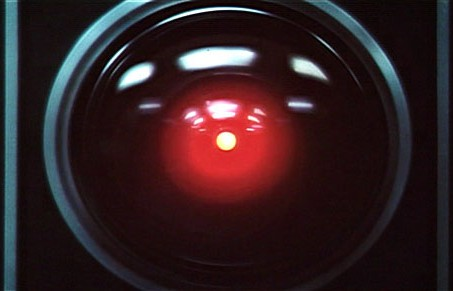
\includegraphics[scale=0.25]{images/hal.jpg}
    \end{figure}
  \end{columns}
\end{frame}


\begin{frame}
  \frametitle{Prosodia}
  \begin{itemize}
    \item El ``cómo'' decimos las cosas, a diferencia del ``qué''
    \item Parte fundamental del mensaje oral
    \item Algunas características que la definen: acentuación, velocidad, tono, ritmo, volumen.
    \item Es justamente en lo principal que fallan los sistemas humano-computadoras hoy día
  \end{itemize}
\end{frame}



\begin{frame}
  \frametitle{Entrainment}

  \begin{enumerate}
    \item Fenómeno también conocido como mimetización, convergencia, efecto camaleón, etc.
    \item Consiste en la adaptación que ocurre entre hablantes a varios niveles: sintáctico, prosódico, en las posturas, etc.
    \item Fenómeno ubícuo e inconsciente en la comunicación humana
  \end{enumerate}

  Recuerden verificarlo en la próxima conversación que tengan
\end{frame}

\begin{frame}
  \frametitle{¿Y cómo lo medimos?}

  \begin{itemize}
    \item La definición de entrainment hasta acá vista es muy subjetiva ¿Cómo definimos una medida para esto?
    \item Vamos a explorar una métrica definida en trabajos anteriores, pulirla un poco, y verificar que efectivamente capture ciertas características del entrainment.
    \item ¿Cómo? Aplicándola a un corpus con anotaciones sociales, y verificando la relación entre las percepciones sociales y la métrica del \emph{entrainment}

  \end{itemize}




\end{frame}
